\documentclass[brazil,times]{abnt}
\usepackage[T1]{fontenc}
\usepackage[utf8]{inputenc}
\usepackage{url}
\usepackage{graphicx}
\usepackage{caption}
\usepackage{subcaption}
\usepackage[pdfborder={0 0 0}]{hyperref}
\usepackage{amssymb}
\usepackage{amsmath}
\usepackage[section]{placeins}
\usepackage{listingsutf8}
\makeatletter
\usepackage{babel}
\makeatother


\lstset{
	language=Octave,
	tabsize=2,
	inputencoding=utf8,
	basicstyle=\scriptsize,
	showspaces=false,
	showstringspaces=false,
	showtabs=false,
}

\begin{document}


\autor{Pedro Paulo Vezzá Campos}

\titulo{Compressão de imagens usando SVD}

\comentario{Terceiro exercício-programa apresentado para avaliação na disciplina
MAC0300, do curso de Bacharelado em Ciência da Computação, turma 45, da
Universidade de São Paulo, ministrada pelo professor Walter Figueiredo Mascarenhas.}

\instituicao{Departamento de Ciência da Computação \par Instituto de Matemática
e Estatística \par Universidade de São Paulo}

\local{São Paulo - SP, Brasil}

\data{\today}

\capa

\folhaderosto

\tableofcontents

\chapter{Introdução\label{cap:introducao}}
	Neste terceiro exercício-programa de MAC0300 - Métodos Numéricos da Álgebra Linear foi pedido que implementássemos um programa que fosse capaz de decompor uma matriz em seus valores singulares (SVD) e aplicar tal algoritmo para a compressão de imagens. Neste relatório serão apresentados: Uma explicação e análise sobre SVD e seus algoritmos (Clássico e Golub-Reinsch), testes realizados e, por fim, será feita apresentada uma conclusão sobre o EP.

% Explique sucintamente o método de Decomposição em Valores Singulares;

% Descreva as principais melhorias do algoritmo implementado para SVD (Golub-Reinsch SVD) de M em relação ao método clássico, que usa os autovalores e autovetores de MMT e MTM.

% Faça a análise da complexidade do algoritmo de SVD implementado (Bidiagonalização de Golub-Kahan e Golub-Reinsch SVD).

% Mostre, para uma determinada imagem em RGB, diferentes compressões variando o valor do rank.



\chapter{Decomposição em Valores Singulares}
	A Decomposição em Valores Singulares (SVD) é uma conhecida fatoração de uma matriz em três termos. Tal decomposição possui várias aplicações, variando desde processamento de sinais até estatística.
	
	Uma SVD é definida para uma matriz M de dimensões $m \times n$ como sendo o produto $$ M = U \Sigma V^T $$ com as seguintes restrições:
	
	\begin{itemize}
		\item $U$ é uma matriz $m \times m$. Suas colunas são conhecidas como \emph{vetores singulares à esquerda} e são autovetores de $MM^T$
		\item $\Sigma$ é uma matriz diagonal. Os valores da diagonal de $\Sigma$ são conhecidos como \emph{valores singulares de M} e são as raízes quadradas dos autovalores diferentes de zero de tanto $M^TM$ quanto $MM^T$.
		\item $V^T$ é uma matriz $n \times n$. Suas colunas são conhecidas como \emph{vetores singulares à direita} e são autovetores de $M^TM$
	\end{itemize}
	
	Para fins deste EP, houve a opção por implementar uma versão da SVD compacta. Nela, nem todos os autovetores são calculados, apenas os necessários para a reconstrução da matriz $M$ a partir dos três fatores. No código implementado, a decomposição é descrita da seguinte forma:
	
	\begin{itemize}
		\item $U$ é $m \times min(m,n)$ e possui colunas ortogonais
		\item S é $min(m,n) \times min(m,n)$ e é uma matriz diagonal contendo na diagonal principal os valores singulares
		\item V é $n \times min(m,n)$ e possui colunas ortogonais
	\end{itemize}

	\section{Algoritmo Clássico}
		A decomposição em valores singulares possui como vantagem o fato que pode ser aplicado a qualquer matriz de dimensões $m \times n$ enquanto a decomposição em autovalores e autovetores só é possível para algumas matrizes quadradas. No entanto, podemos traçar paralelos entre ambas decomposições.
		
		Dada uma SVD de uma matriz M, temos que:
		
    	$$M^{T} M = V \Sigma^{T} U^{T}\, U \Sigma V^{T} = V (\Sigma^{T} \Sigma) V^{T}\,$$
    	$$M M^{T} = U \Sigma V^{T} \, V \Sigma^{*} U^{T} = U (\Sigma \Sigma^{T}) U^{T}.\,$$
	
		As expressões que se encontram no lado direito das igualdades descrevem decomposições em autovalores e autovetores das expressões do lado esquerdo. Isso traz como consequência que:
		
		\begin{itemize}
			\item As colunas de $V$ são autovetores de $M^{T}M$.
			\item As colunas de $U$ são autovetores de $MM^{T}$.
			\item Os valores diferentes de zero de $\Sigma$ são as raizes quadradas dos autovalores diferentes de zero de $M^{T}M$ ou $MM^{T}$.
		\end{itemize}
		
		Este algoritmo para a obtenção da decomposição em valores singulares funciona corretamente para matrizes menores e quando os valores singulares são significativamente maiores que a precisão adotada nos cálculos. Por outro lado, há uma perda de precisão inerente ao algoritmo que será explicado na \ref{melhorias}, o que nos induz a buscar um algoritmo que não faça uso do cálculo de autovalores e autovetores de $M^{T}M$, que será apresentado na seção \ref{golub-reinsch}.

	\section{Algoritmo de Golub-Reinsch\label{golub-reinsch}}
		O Algoritmo de Golub-Reinsch é um método que faz uso extensivo de rotações e reflexões para obter a SVD sem calcular $M^{T}M$, o que poderia trazer problemas como será apresentado em seguida.
		O processo é dividido em duas etapas. Na primeira fase devemos reduzir a matriz $M$ original à forma bidiagonal utilizando reflexões de Householder aplicadas alternadamente à esquerda para zerar as colunas abaixo da diagonal principal e à direita para zerar linhas acima da superdiagonal.
		A segunda fase é a computação propriamente dita da SVD. Através de rotações de Givens vamos iterativamente zerando os elementos da superdiagonal enquanto acumulamos as rotações realizadas nas matrizes $U$ e $V$. Este processo é repetido enquanto não for atingida uma precisão maior que uma especificada (O $\epsilon$ da máquina por exemplo). 
		
	\section{Análise de Complexidade do Algoritomo de Golub-Reinsch}
		\subsection{Primeira Fase: Bidiagonalização de Golub-Kahan}
			Como vamos aplicando refletores alternadamente à esquerda e à direita, ao final da primeira fase do cálculo da SVD são necessários $n$ refletores à esquerda e $n - 2$ refletores à direita. Podemos traçar um paralelo entre o processo de bidiagonalização e o de aplicar duas fatorações QR de Householder entrelaçadas, a primeira operando na matriz $M$ de dimensões $m \times n$ e a outra operando na matriz $M^{T}$ de dimensões $n \times m$. Assim, o custo total para a bidiagonalização é de $\sim 4mn^2 - \frac{4}{3}n^3$ flops. \cite{trefethen}
		\subsection{Segunda Fase: Golub-Reinsch SVD}
			Na segunda fase a princípio seria necessário um número infinito de rotações de Givens para que a matriz $\Sigma$ convirja a uma matriz diagonal. Porém, a convergência é superlinear e em $O(n log(|log(\epsilon)|))$ iterações atingimos a precisão $\epsilon$ da máquina. Na prática, sendo $\epsilon$ uma constante, a convergência é dada em $O(n)$ iterações. Ainda, como a matriz é originalmente bidiagonal, são necessários apenas $O(n)$ flops por iteração, totalizando $O(n^2)$ flops para a segunda fase. Como conclusão, na prática, a primeira fase do algoritmo de Golub-Reinsch é assintoticamente mais custosa que a segunda, ditando a complexidade final do algoritmo. \cite{trefethen}
			

	\section{Melhorias do Algoritmo de Golub-Reinsch ao Método Clássico\label{melhorias}}
		Apesar do algoritmo clássico ser relativamente barato computacionalmente ele possui como problema o fato que valores singulares pequenos serão calculados de maneira imprecisa. Isto é uma consequência do efeito de ``perda de informação através da elevação ao quadrado'' que acontece quando calculamos $M^{T}M$ a partir de $A$.
		
		Nós podemos ter uma ideia desta perda de informação ao considerar um exemplo. Suponha que as entradas da matriz A são conhecidas com exatidão em seis casas decimais. Se A tem, digamos $\sigma_1 \approx 1$ e $\sigma_{17} \approx 10^{-3}$, então $\sigma_{17}$ é razoavelmente menor que $\sigma_1$, mas ainda assim acima da precisão de $\epsilon \approx 10^{-5}$ ou $10^{-6}$. Nós gostaríamos de calcular $\sigma_{17}$ com talvez duas ou três casas de precisão. As entradas de $M^{T}M$ tem também precisão de aproximadamente volta de seis casas decimais. Associada com os valores singulares $\sigma_1$ e $\sigma_{17}$, $M^{T}M$ tem autovalores $\lambda_1 = \sigma_{1}^{2} \approx 1$ e $\lambda_{17} = \sigma_{17}^{2} \approx 10^{-6}$. Note que $\lambda_{17}$ tem a mesma magnitude que os erros nas entradas de $M^{T}M$. Portanto não podemos esperar que $\lambda_{17}$ possa ser calculado de maneira precisa. \cite{watkins2004fundamentals}
	
	
\chapter{Testes Realizados}
	Como foi pedido no enunciado, o algoritmo implementado foi utilizado para comprimir uma imagem RGB ao alterarmos o número do posto (\emph{rank}) da decomposição obtida escolhendo apenas as $k$ primeiras colunas de $U$, linhas e colunas de $\Sigma$ e colunas de $V$. Os resultados condizem com o esperado, estando os valores singulares ordenados, os primeiros possuem um ``peso'' maior na composição da imagem final. O efeito prátio é que com uma quantidade menor de termos na série que define a matriz da imagem original a partir da SVD podemos montar uma imagem comprimida muito próxima da original.
	
	\begin{figure}[hb]
		\centering
		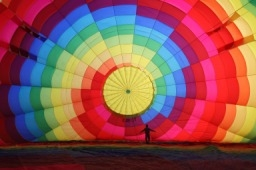
\includegraphics[scale=1]{imagens/balloon256.jpg}
		\caption[Imagem original] {Imagem original ($256 \times 170$)}
	\end{figure}
	
	\begin{figure}
        \centering
        \begin{subfigure}[b]{0.5\textwidth}
                \centering
                
\includegraphics[width=\textwidth]{imagens/balloon256-compressed-1.jpg}
                \caption{$k = 1$}
        \end{subfigure}%
        ~ %add desired spacing between images, e. g. ~, \quad, \qquad etc. 
          %(or a blank line to force the subfigure onto a new line)
        \begin{subfigure}[b]{0.5\textwidth}
                \centering
                
\includegraphics[width=\textwidth]{imagens/balloon256-compressed-2.jpg}
                \caption{$k = 2$}
        \end{subfigure}

        \begin{subfigure}[b]{0.5\textwidth}
                \centering
                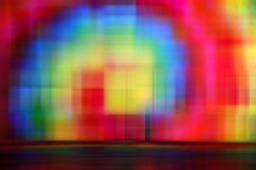
\includegraphics[width=\textwidth]{imagens/balloon256-compressed-4.jpg}
                \caption{$k = 4$}
        \end{subfigure}%
        ~ %add desired spacing between images, e. g. ~, \quad, \qquad etc. 
          %(or a blank line to force the subfigure onto a new line)
        \begin{subfigure}[b]{0.5\textwidth}
                \centering
                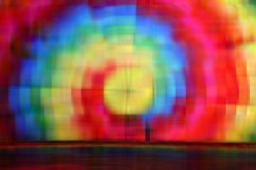
\includegraphics[width=\textwidth]{imagens/balloon256-compressed-8.jpg}
                \caption{$k = 8$}
        \end{subfigure}
        
                \begin{subfigure}[b]{0.5\textwidth}
                \centering
                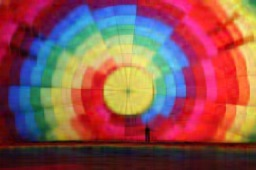
\includegraphics[width=\textwidth]{imagens/balloon256-compressed-16.jpg}
                \caption{$k = 16$}
        \end{subfigure}%
        ~ %add desired spacing between images, e. g. ~, \quad, \qquad etc. 
          %(or a blank line to force the subfigure onto a new line)
        \begin{subfigure}[b]{0.5\textwidth}
                \centering
                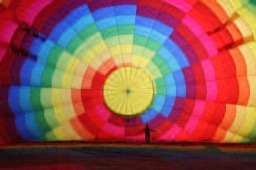
\includegraphics[width=\textwidth]{imagens/balloon256-compressed-32.jpg}
                \caption{$k = 32$}
        \end{subfigure}

        \begin{subfigure}[b]{0.5\textwidth}
                \centering
                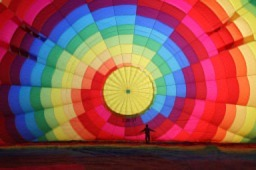
\includegraphics[width=\textwidth]{imagens/balloon256-compressed-64.jpg}
                \caption{$k = 64$}
        \end{subfigure}%
        ~ %add desired spacing between images, e. g. ~, \quad, \qquad etc. 
          %(or a blank line to force the subfigure onto a new line)
        \begin{subfigure}[b]{0.5\textwidth}
                \centering
                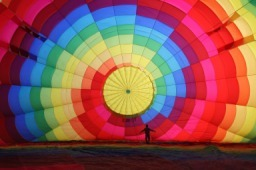
\includegraphics[width=\textwidth]{imagens/balloon256-compressed-128.jpg}
                \caption{$k = 128$}
        \end{subfigure}

        \caption{Resultado das compressões para diferentes valores de $k$}
	\end{figure}

	
	
\chapter{Conclusão}
	Neste trabalho foram apresentados uma explicação sucinta sobre a decomposição em valores singulares (SVD). Posteriormente, foram vistos dois algoritmos distintos para obter tal decomposição e, em seguida, uma comparação foi traçada entre a eficácia de cada um dos métodos juntamente com uma análise de complexidade do algoritmo de Golub-Reinsch. Por fim, foram apresentados resultados experimentais do método de compressão de imagens apresentado no enunciado do EP.
	
	O trabalho inovou ao introduzir aos alunos de Ciência da Computação a uma vasta área dentro do ramo que é a compressão de dados, tão relevante frente à crescente demanda, por exemplo, de conteúdos multimídia com resolução cada vez maior. Desta vez, a fundamentação teórica não é tão complexa depois que os alunos já estão habituados a conceitos como decomposições QR de Givens, Householder, autovalores e autovetores. Porém, a carga de programação foi bem mais intensa que antes, o algoritmo de Golub-Reinsch tem muitas subrotinas que devem ser implementadas.
	
\nocite{*}
\bibliographystyle{abnt-num}
\bibliography{bibliografia}
\end{document}

\end{document}
